\documentclass[14pt]{extarticle}
\usepackage{fontspec}
\setmainfont{Times New Roman}
\usepackage{polyglossia}
\setmainlanguage{russian}
\usepackage{indentfirst}
\usepackage{array}
\usepackage{booktabs}
\usepackage{siunitx}
\sisetup{
	output-decimal-marker={,},
	exponent-product=\cdot,
	per-mode=symbol
}

\setlength{\parindent}{1.25cm}
\setlength{\parskip}{0pt}
\usepackage{graphicx}
\usepackage{float}

\title{Техническое задание: Симулятор гравитационного взаимодействия}
\author{Арсен Джабраилов}

\begin{document}
	
	\maketitle
	
	\section{Цель}
	Визуализация эволюции системы космических объектов под действием гравитации через три ортогональные 2D-проекции (XY, XZ, YZ) и таблицу координат.
	
	\section{Границы}
	
	\subsection{Включено}
	\begin{itemize}
		\item Точечные массы в форме однородных шаров
		\item Гравитация по Ньютону%: $F = G \cdot \frac{m_1 \cdot m_2}{r^2}$, где $G = \num{6.67430e-11}$ м³/(кг·с²)
		\item Интегратор Верле
		\item Столкновения твёрдых тел: слияние / распад на частицы
		\item Предел Роша с временным условием
		\begin{itemize}
			\item Нет приливной деформации формы, объект не разрушается частично от приливных сил: он либо цел, либо сломан
			\item Разрушение происходит только после пребывания внутри предела Роша не менее 24 часов
		\end{itemize}
		\item СИ
		\begin{itemize}
			\item Масса --- кг
			\item Расстояние --- м
			\item Время --- с
		\end{itemize}
	\end{itemize}
	
	\subsection{Исключено}
	\begin{itemize}
		\item Вращение тел вокруг оси
		\item Релятивистские эффекты, магнитные поля, приливная деформация формы
		\item Сложные космические объекты (такие как чёрные дыры, звёзды, газовые гиганты)
		\item Фрагментация осколков (осколки не могут разрушаться повторно)
	\end{itemize}
	
	\subsection{Ограничения на параметры объектов}
	\begin{table}[H]
		\centering
		\begin{tabular}{l S[table-format=1.3e2] S[table-format=1.1e2] p{5.5cm}}
			\toprule
			Параметр & {Минимум} & {Максимум} & Обоснование \\
			\midrule
			Масса & e15 & e26 & Нижняя граница --- избежание потери чисел при расчётах с большой разницей порядков; верхняя граница --- предел твёрдых тел \\
			& {\footnotesize (\num{0.1} $M_{\text{Л}}$)} & {\footnotesize (\num{100} $M_{\odot}$)} & \\
			\midrule
			Радиус & e3 & 2.0e7 & Нижняя граница --- избежание сингулярностей; верхняя граница --- предел твёрдых тел \\
			& {\footnotesize (\num{0.1} $R_{\text{Л}}$)} & {\footnotesize (\num{10} $R_{\odot}$)} & \\
			\midrule
			Кол-во объектов & 0 & e5 & Пользователь может уменьшить ограничение при необходимости; большее число объектов вызовет большую нагрузку.\\
			\bottomrule
		\end{tabular}
		\caption{Допустимые диапазоны параметров объектов}
	\end{table}
	
	\subsection{Ограничения на фрагментацию}
	\begin{itemize}
		\item Объект может разрушиться только если его масса $\ge$ \num{2e15} кг (в 2 раза больше минимальной)
		\item Число фрагментов для одного объекта --- 2--100 (настраивается пользователем)
		\item Если при разрушении общее число объектов превысит 10000, создаётся только допустимое число осколков
		\item Осколки не могут фрагментироваться повторно
	\end{itemize}
	
	\subsection{Правила столкновений твёрдых тел}
	При контакте двух объектов (расстояние $\le R_1 + R_2$) результат определяется соотношением масс и относительной скоростью:
	
	\begin{table}[H]
		\centering
		\begin{tabular}{l l p{6cm}}
			\toprule
			Соотношение масс $\frac{m_{\min}}{m_{\max}}$ & Условие & Результат \\
			\midrule
			$< \frac{1}{100}$ & --- & Слияние: два объекта сливаются в один \\
			\midrule
			$\frac{1}{100} \leq r < \frac{1}{10}$ & Случайный выбор & Поглощение или разрушение (вероятность разрушения прямо пропорциональна соотношению масс) \\
			\midrule
			$\geq \frac{1}{10}$ & $v_{\text{rel}} > v_{\text{esc}}$ & $\Rightarrow$ Распад на фрагменты \\
			& $v_{\text{rel}} \leq v_{\text{esc}}$ & $\Rightarrow$ Слияние\\
			\bottomrule
		\end{tabular}
		\caption{Правила обработки столкновений}
	\end{table}
	
	где:
	\begin{itemize}
		\item $v_{\text{rel}} = |\vec{v_1} - \vec{v_2}|$ --- относительная скорость в момент контакта
		\item $v_{\text{esc}} = \sqrt{\frac{2 \cdot G \cdot m_{\min}}{R_{\min}}}$ --- вторая космическая скорость меньшего объекта
	\end{itemize}
	
	\subsection{Правила предела Роша}
	\begin{itemize}
		\item Формула предела Роша:
		\[
		d_{\text{Roche}} = 2.9 \cdot R_{\text{primary}} \cdot \sqrt[3]{\frac{\rho_{\text{primary}}}{\rho_{\text{satellite}}}}
		\]
		\item Разрушение происходит только если объект пребывает внутри предела Роша $\ge$ 24 часов
		\item При разрушении создаётся 4--100 фрагментов (настраивается пользователем)
		\item Масса каждого фрагмента = $\frac{m_{\text{parent}}}{N_{\text{fragments}}}$
		\item Каждый фрагмент сферический
	\end{itemize}
	
	\section{Функционал}
	
	\subsection{Формат входных данных}
	Для каждого объекта задаются следующие параметры:
	\begin{itemize}
		\item имя (строка),
		\item масса (вещественное число),
		\item радиус (вещественное число),
		\item положение в пространстве (3 вещественных числа),
		\item вектор скорости (3 вещественных числа),
		\item вектор ускорения (3 вещественных числа),
	\end{itemize}
	
	Объекты не могут иметь одинаковые имена. Фрагменты наследуют имя родителя с суффиксом --- индивидуальным номером осколка.
	
	При загрузке готового сценария используется формат файла .csv.
	
	\subsection{Включено}
	\begin{itemize}
		\item Возможность создать свой объект
		\item Возможность загрузить готовый шаблон или объект реального мира
		\item Возможность сохранения сценария в CSV файл
		\item Возможность загрузки сценария в виде CSV файла
		\item Три ортогональные 2D-проекции
		\item Таблица с координатами/скоростями/ускорениями
		\item Возможность изменения скорости симуляции, её приостановки или перезапуска
		\item Настройка числа фрагментов (2--100) через интерфейс
	\end{itemize}
	
	\subsection{Исключено}
	\begin{itemize}
		\item Drag \& Drop
		\item Возможность загрузки новых объектов во время симуляции
		\item 3D-рендеринг
	\end{itemize}
	
	\subsection{Пример интерфейса}
	\begin{figure}[H]
		\centering
		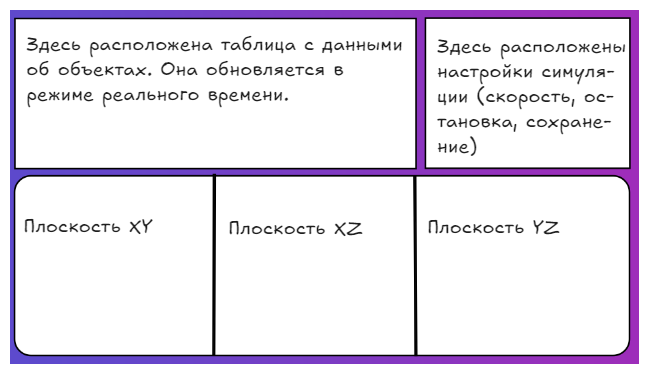
\includegraphics[width=0.85\linewidth]{interface.png}
		\caption{Пример интерфейса программы}
		\label{fig:drawing-2026-02-08-15}
	\end{figure}
	
	
	\section{Технологии}
	Python.%, PNG-текстуры.
	
\end{document}